\documentclass[12pt]{article}
\usepackage{sbc-template}
\usepackage{graphicx,url}
\usepackage[brazil]{babel}
\usepackage[utf8]{inputenc}
\usepackage{amssymb}
\usepackage{amsmath}

\sloppy

\title{Uma investigação quanto à Lógica Difusa e suas aplicações}

\author{Fernando Concatto\inst{1}}

\address{Bacharelado em Ciência da Computação -- Universidade do Vale do Itajaí (UNIVALI) \\
  Caixa Postal 360 -- CEP 88302-202 -- Itajaí -- SC -- Brasil
  \email{fernandoconcatto@edu.univali.br}
}

\begin{document}

\maketitle

\begin{abstract}
  Traditional mathematical sets display profoundly binary characteristics, a property that rarely accomodates real situations that involve imprecision and uncertainty. In this context, the Fuzzy Logic model was developed, which allows elements to exhibit partial membership to a set. This work intended to identify the fundamental concepts of Fuzzy Logic, describing the particularities of this novel notion of sets, and also to present practical applications of this model of logic.
\end{abstract}

\begin{resumo}
  Conjuntos matemáticos tradicionais apresentam características profundamente binárias, uma propriedade que raramente acomoda situações reais que envolvem imprecisão e incerteza. Nesse contexto, o modelo de Lógica Difusa foi desenvolvido, que permite pertinência parcial de objetos a um conjunto. Este trabalho buscou identificar os conceitos fundamentais da Lógica Difusa, descrevendo as particularidades desta nova noção de conjuntos e as operações entre eles, além de apresentar aplicações práticas deste modelo de lógica.
\end{resumo}

\section{Introdução} \label{sec:intro}

A lógica tradicional, desenvolvida inicialmente pelo filósofo grego Aristóteles, é marcada por conceitos fortemente binários. Um princípio que evidencia essa noção é a Lei do Terceiro Excluído, uma das clássicas leis do pensamento, que estabelece que toda proposição é verdadeira ou sua negação é verdadeira; não há nenhum estado intermediário. Entretanto, devido à frequência com que a incerteza e a imprecisão se fazem presentes no estudo de sistemas complexos, foi identificada a carência de um modelo lógico que lide com essas características \cite{Ross2010}.

A noção de imprecisão é inerente ao raciocínio humano. Muito frequentemente, quando uma decisão casual deve ser tomada, aproximações são empregadas ao invés de medidas exatas. Um exemplo dessa situação é a decisão de quantos gramas de café e quantos litros de água serão utilizados na preparação de uma garrafa de café; geralmente, medidas aproximadas como três colheres ou dois copos são empregadas nessas circunstâncias. Categorias exibem esse mesmo fenômeno: ``música de rock'', por exemplo, não possui uma definição exata, mas indivíduos geralmente conseguem decidir facilmente se uma música pertence ou não ao gênero.

Perante estas circunstâncias, o cientista azerbaijano Lofti Zadeh propôs em 1965 o sistema de Lógica Difusa, onde elementos podem pertencer parcialmente a um conjunto, ao invés de apenas pertencerem ou não pertencerem. Este trabalho visa investigar o sistema de Lógica Difusa, apresentando seus fundamentos e analisando suas aplicações nos diversos campos da ciência e engenharia.

\section{Fundamentos da Lógica Difusa} \label{sec:fundaments}

A Lógica Difusa é composta por diversos conceitos fundamentais. Um dos conceitos que mais se fazem presentes na proposição de Zadeh é ideia de conjuntos difusos, que permitem pertinência parcial de elementos, ao invés de apenas inclusão ou exclusão. Associadas a estes conjuntos estão as variáveis linguísticas, que descrevem valores de maneira textual ao invés de estritamente numérica. Esta seção descreve detalhadamente estes conceitos, apresentando noções relacionadas e exemplos de utilização.

\subsection{Conjuntos difusos}

A noção de \textit{conjuntos difusos} é essencial para a Lógica Difusa. Zadeh os descreve como conjuntos onde objetos podem pertencer parcialmente ao conjunto, ao contrário de conjuntos clássicos, que possuem uma definição formal e absolutamente precisa. O conceito tradicional de conjuntos estabelece que um objeto está ou não está no conjunto, necessariamente desconsiderando qualquer posição intermediária. Desta forma, é impossível propôr que um objeto esteja ``fortemente'' ou ``fracamente'' presente em um determinado conjunto; o objeto simplesmente percente ou não.

A contraposição a essa característica dos conjuntos clássicos é o ponto chave da Lógica Difusa. Conjuntos difusos apresentam níveis de pertinência, definidos a partir de valores no intervalo $[0, 1]$. Desta maneira, é possível descrever quão fortemente um objeto pertence a um conjunto, com valores próximos a 0 representando elementos que possuem uma presença fraca no conjunto e valores próximos a 1 indicando elementos que pertencem de forma significativa ao conjunto. Os valores 0 e 1 equivalem aos conjuntos clássicos, denotando que o objeto não pertence ou percente ao conjunto, respectivamente. A função que descreve esse nível de pertinência é chamada de \textbf{função de pertinência}, do inglês \textit{membership function} \cite{Zadeh1965}. Um exemplo de função de pertinência de forma triangular é apresentada na figura \ref{fig:membership}; outras formas típicas para a função de pertinência são a trapezoide e a gaussiana.

\begin{figure}[ht]
    \centering
    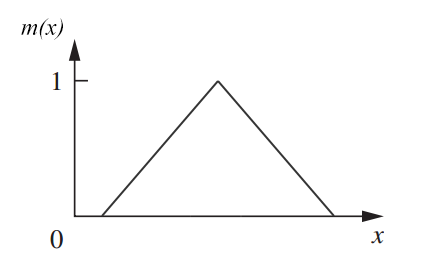
\includegraphics[width=8cm]{membership.png}
    \caption{Função de pertinência triangular.}
    \label{fig:membership}
\end{figure}

\subsection{Variáveis linguísticas e Fuzzificação} \label{sec:linguisticvars}

Um conceito adicional crucial para a Lógica Difusa, relacionado com os conjuntos difusos, é o de \textit{variáveis linguísticas}. Introduzidas por Zadeh em 1975, variáveis linguísticas possuem um propósito bastante similar às variáveis numéricas convencionais, com a diferença primordial de que seus valores são representados por palavras ao invés de números. Desta maneira, para uma variável ``idade'', o conceito clássico de variáveis poderia exibir números de 1 a 100, enquanto a noção linguística apresentaria valores como \textit{jovem}, \textit{velho} ou \textit{muito velho}, entre outras denominações \cite{Zadeh1975}.

Valores de uma variável linguística são tratados como conjuntos difusos, e portanto possuem uma função de pertinência que determina o grau de verdade (no intervalo $[0, 1]$) de um argumento contável. Por exemplo, para o valor linguístico \textit{velho} da variável ``idade'', o argumento 50 anos poderia apresentar um grau de verdade de $0.5$; já para uma variável de nome ``clima'', uma temperatura de 35 $^{\circ}$C para o valor linguístico \textit{quente} poderia exibir um grau de verdade de $0.9$. Este processo de conversão de um valor de entrada para o nível de pertinência a um conjunto difuso é chamado de \textbf{fuzzificação}, do inglês \textit{fuzzification}, e compõe o primeiro passo da execução de um sistema de inferência baseado em Lógica Difusa, detalhado na seção \ref{sec:inference}.

\section{Operações entre conjuntos difusos} \label{sec:operations}

Conjuntos clássicos apresentam três operadores fundamentais: união, intersecção e complemento, sendo a união e a interseção operadores binários e o complemento um operador unário. A \textbf{união} entre dois conjuntos A e B é composta pelos elementos que estão em A ou em B, sem repetições. A \textbf{intersecção} entre dois conjuntos A e B é constituída pelos elementos que estão tanto em A quanto em B. O \textbf{complemento} de um conjunto A é composto por todos os elementos que \textit{não} estão em A \cite{Houston2009}.

Conjuntos difusos também apresentam estes operadores, porém com formulações diferentes, para acomodar as particularidades da Lógica Difusa. Como a noção de pertinência em conjuntos difusos é estabelecida por valores no intervalo $[0, 1]$, os operadores são definidos em termos da função de pertinência $m(x)$ do conjunto. A união entre dois conjuntos difusos A e B é definida pelo maior valor entre as duas funções de pertinência $m_{A}(x)$ e $m_{B}(x)$, enquanto que a intersecção é definida pelo menor valor entre elas. O complemento de um conjunto difuso A é definido por $1 - m_{A}(x)$, invertendo o formato da função \cite{Zadeh1965}.

Estas definições se mostram bastante condizentes com as características dos operadores em conjuntos clássicos. No caso da união, a função de pertinência do conjunto difuso resultante apresentará um formato ``maior'', que contém as funções dos conjuntos que foram unidos. Para a intersecção, o formato será ``pequeno'', representando apenas as áreas onde as duas funções estão sobrepostas. As figuras \ref{fig:union} e \ref{fig:intersection} demonstram essas características, evidenciando uma forte similaridade com os diagramas de Venn.

\begin{figure}
    \centering
    \begin{minipage}{0.45\textwidth}
        \centering
        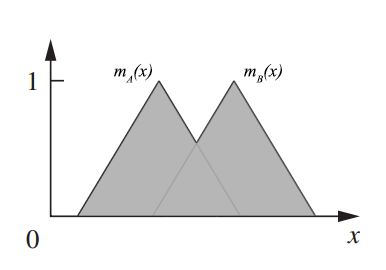
\includegraphics[width=1.1\textwidth]{union.png}
        \caption{União.}
        \label{fig:union}
    \end{minipage}\hfill
    \begin{minipage}{0.45\textwidth}
        \centering
        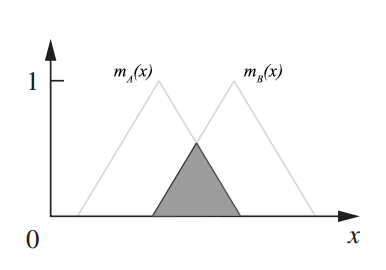
\includegraphics[width=1.1\textwidth]{intersection.png}
        \caption{Intersecção.}
        \label{fig:intersection}
    \end{minipage}
\end{figure}

\section{Sistemas de inferência} \label{sec:systems}

Sistemas de inferência utilizando Lógica Difusa foram inicialmente propostos por Mamdani, em 1975, em uma tentativa de implementar um sistema de controle linguístico para motores a vapor em uma fábrica. Estes sistemas utilizam uma base de regras, definidas através de cláusulas \textbf{se-então} sobre variáveis linguísticas para tomar decisões a partir de dados de entrada numéricos \cite{Mamdani1975}. O principal atrativo destes sistemas é a capacidade de lidar com situações imprecisas de forma conveniente, devido à utilização dos conceitos de Lógica Difusa.

Crucialmente, as regras de um sistema de inferência são especificadas em termos linguísticos, facilitando a sua especificação por um especialista no domínio do problema. Por exemplo, para um sistema de controle de ar condicionado, uma das regras poderia assumir a seguinte forma: \textbf{se} temperatura está quente \textbf{então} aumente a potência do ar condicionado. Neste caso, quente é um dos valores da variável linguística temperatura. É possível também utilizar os operadores lógicos \textit{e}, \textit{ou} e \textit{não}, que são implementados através dos operadores de intersecção, união e complemento, respectivamente.

Adicionalmente, para todos os valores das variáveis linguísticas (representados por conjuntos difusos), uma função de pertinência deve ser especificada. Essa função mapeará valores contáveis para níveis de pertinência ao conjunto, como exemplificado na seção \ref{sec:linguisticvars}. As regras do sistema de inferência são aplicadas sobre esses níveis de pertinência.

\subsection{Fuzzificação} \label{sec:fuzzification}

A operação de transformação de valores numéricos para conjuntos difusos é denominada \textbf{fuzzificação}, e compõe o primeiro passo de um sistema de inferência. Este processo avalia a pertinência de um valor de entrada $x$ a um conjunto difuso $A$ através da função de pertinência $m_{A}(x)$. O sistema pode conter mais de um valor de entrada; neste caso, todos os níveis de pertinência são computados. Então?, o conjunto a qual o valor de entrada pertence e o nível de pertinência são passados para estágio de inferência, descrito adiante.

\subsection{Inferência} \label{sec:inference}

A inferência compõe o segundo estágio de um sistema de controle por Lógica Difusa. Este passo utiliza a base de regras do sistema para transformar os dados de entrada em alguma ação concreta. Existem diversos métodos para efetuar esse processo, como o de Mamdani \cite{Mamdani1975} e de Sugeno \cite{Sugeno1988}, cada um com algumas variações específicas. O método de Mamdani é descrito a seguir.

Para cada regra aplicável aos dados recebidos do estágio de fuzzificação, a \textit{força} ou \textit{aceitação} da regra é calculada. Este valor é calculado primeiramente limitando (truncando) as funções de pertinência de cada conjunto aplicável (definidos pela porção \textbf{se} da regra) ao nível de pertinência do valor de entrada. Na sequência, caso a regra especifique operações lógicas entre os conjuntos de entrada, os mesmos são combinados utilizando as técnicas descritas na seção \ref{sec:operations}. O valor resultante é a força de regra, no intervalo $[0, 1]$.

%Imagens!!!

Em seguida, a função de pertinência do conjunto de saída (porção \textbf{então} da regra) é limitada à força da regra, gerando a função de pertinência $m_{S}(x)$ do conjunto resultante $S$. Os conjuntos difusos resultantes das regras aplicáveis representam a ação a ser tomada, e são transferidos ao estágio final do sistema, descrito na sequência, como um único conjunto difuso, agregado a partir da união de todos os conjuntos.

\subsection{Defuzzificação} \label{sec:defuzzification}

O processo de \textbf{defuzzificação}, do inglês \textit{defuzzification}, envolve a conversão do conjunto difuso gerados pelo estágio de inferência de volta para um valor numérico, para que possa ser aplicado no contexto do sistema sendo controlado. Diversos métodos foram desenvolvidos para realizar a defuzzificação de conjuntos difusos; os mais utilizados entre eles são o \textit{método da média dos máximos} e \textit{método do centroide} \cite{Ross2010}.

O método da média dos máximos é uma técnica computacionalmente simples, que envolve o cálculo da média entre os pontos $a$ e $b$ que representam o início e o término da região onde a função de pertinência apresenta o valor máximo. O valor resultante $z$ é calculado pela expressão \ref{eq:mom}.

\begin{equation}
  \label{eq:mom}
  z = \frac{a + b}{2}
\end{equation}

O método do centroide se trata de uma técnica muito mais sofisticada, porém custosa. Envolve o cálculo do ponto central da área representada pela função de pertinência $m_{S}(x)$ do conjunto difuso $S$, utilizando integração algébrica. Este ponto é calculado através da expressão .

\begin{equation}
  \label{eq:centroid}
  z = \frac{\int m_{S}(x) \cdot x \; dx}{\int m_{S}(x) \; dx}
\end{equation}

\section{Aplicações da Lógica Difusa} \label{sec:applications}

Lorem ipsum dolor sit amet, consectetur adipisicing elit, sed do eiusmod tempor incididunt ut labore et dolore magna aliqua. Ut enim ad minim veniam, quis nostrud exercitation ullamco laboris nisi ut aliquip ex ea commodo consequat. Duis aute irure dolor in reprehenderit in voluptate velit esse cillum dolore eu fugiat nulla pariatur. Excepteur sint occaecat cupidatat non proident, sunt in culpa qui officia deserunt mollit anim id est laborum.

\bibliographystyle{sbc}
\bibliography{bibliography}

\end{document}
